

TODO: NACH TODO SUCHEN!!!!!!!!!!!!!!!!!!!!!!!!!!!!!!!!!!!!!!!!!!!!!!!!!!!!!!!!

!!!!!!!!!!!!!!!!!!!!!!!!!!!!!!!

!!!!!!!!!!!!!!!!!!!!!!!!!!!!!!!

!!!!!!!!!!!!!!!!!!!!!!!!!!!!!!!

!!!!!!!!!!!!!!!!!!!!!!!!!!!!!!!

!!!!!!!!!!!!!!!!!!!!!!!!!!!!!!!\\

!!!!!!!!!!!!!!!!!!!!!!!!!!!!!!!

!!!!!!!!!!!!!!!!!!!!!!!!!!!!!!!

!!!!!!!!!!!!!!!!!!!!!!!!!!!!!!!

!!!!!!!!!!!!!!!!!!!!!!!!!!!!!!!






\section{Technische Hintergründe}

\subsection{Geschichte des Ext-Dateisystems}

% TODO: hier bissl mehr?
% TODO: RE-READ ALLES FREITAG!!!!!!!!!!!!!!!
% TODO: AUCH GLEICH BLOG POST! mit paar screenshots vielleicht?

Das sogenannte \ac{ext} war das Erste einer Reihe von Dateisystemen welches speziell für Linux entwickelt wurde und damals das minix-Dateisystem ablöste. \ac{ext} in Version 1 ist mittlerweile allerdings veraltet und wird in aktuellen Linux-Distributionen nicht mehr verwendet. Ext3 ist die neuere Variante, bleibt von Grund auf jedoch exakt gleich wie Ext2, führt jedoch "file system journaling" ein. Die folgenden Varianten sind aktuell noch gängig und werden aktiv eingesetzt:

\begin{itemize}
	\item ext2 - Führte separate Zeitstempel für Dateizugriffe, Inode- und Datenmodifikation ein. Bringt keine Unterstützung für journaling.
	\item ext3 - Führte journaling ein (und ist required!)
	\item ext4 - Unterstützung für fast fsck, native filesystem encryption, journaling, jedoch auch für non-journaling
\end{itemize}

% TODO


\subsection{Basics}

Das Ext-Dateisystem verwendet Blöcke als Basiseinheit zum Speichern von Daten \cite{Ext2.07.01.2022}. Sogenannte "Inodes (Index-Nodes) werden zum Speichern von Metadaten verwendet, Blockgruppen zur optimierten logischen Strukturierung, Verzeichnisse um hierarchische Strukturen darstellen zu können, Block- und Inode-Bitmaps um allokierte Blöcke und Inodes zu kennzeichnen, sowie Superblöcke um allgemeine Informationen des Dateisystems zu speichern. Kopien von wichtigen Datenstrukturen wie z.B. den Superblöcken werden redundant vorgehalten und alle Daten welche mit Dateien assoziiert werden, sind aus Gründen der Performance gut lokalisiert\cite{Carrier.06.01.2022}.

\begin{figure}[H]
	\centering
	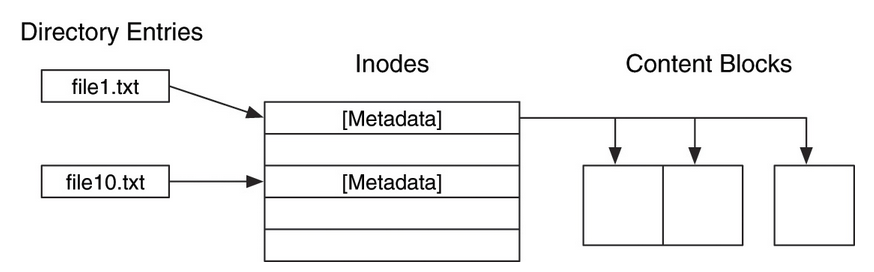
\includegraphics[width=12cm,keepaspectratio=true]{pictures/ext1.png}
	\caption{
		Zusammenhang zwischen Verzeichniseinträgen, Inodes und Inhaltsblöcken \cite{Carrier.06.01.2022}
	}
	\label{fig:ext2}
\end{figure}

Abbildung \ref{fig:ext2} zeigt blaaaa TODO


% HIER NUN ERSTMAL alle *DEFINITIONS* DURCH!!!!!!!!!!!

\textbf{Praktische Beispiele}

Alle praktischen Beispiele zu diesem Dokument wurden unter Ubuntu (Version 20.04.1) auf einem 32GB USB Stick durchgeführt und hier völlig transparent, je nach Kontext, präsentiert und sollten somit - unter Berücksichtigung selber OS Voraussetzungen - 1-zu-1 nachgemacht werden können. 

Als erstes wurde der USB Stick mit dem Ext3 Dateisystem frisch formatiert:

\begin{lstlisting}[language=bash,caption={Create the FS}]
# find mounted devices and their paths:
lsblk

# unmount the device: (The usb stick here is "/dev/sdc1")
sudo umount /dev/sdc1

# Create the filesystem:
sudo mkfs -t ext3 /dev/sdc
\end{lstlisting}  

\begin{figure}[H]
	\centering
	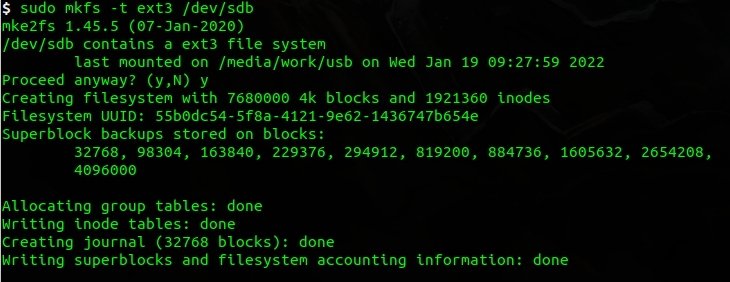
\includegraphics[width=12cm,keepaspectratio=true]{pictures/createfs.png}
	\caption{
		Erstellen eines EXT3 Dateisystems auf einem USB Stick
	}
	\label{fig:createfs}
\end{figure}

Im Abbildung \ref{fig:createfs} ist zu sehen wie das Dateisystem auf dem USB Stick unter "/dev/sdc" erstellt wird. Es werden 7680000 4KB Blöcke mit 1921360 Inodes erstellt (32GB). Für das Dateisystem wird eine \ac{uuid} generiert, ein Journal erstellt, sowie die Blöcke der Superblock-Backups ausgegeben.

% TODO: hier die Superblock analyse erstmal um das alles zu bestätigen!

Writing inode tables:  48/235
WAS SIND inode TABLES!!?!??!?!?!?! 1921360 inodes in 235 tables?!?! NOPE. 235 Block Groups - SEE meine Zeichnung auf Schmierzettel!
1921360 / 235
8176 inodes per BLOCK GROUP
\\

\subsection{Wie speichert das Dateisystem Daten (Inhaltsdaten)?}


ZeichnungEN schmierzettel und mehr! hier nochmal paar Zeichnungen schön hübsch rein, CONTENT!



\subsection{Wie speichert das Dateisystem Metadaten (Dateinamen, Größe, Berechtigungen, Zeitstempel, ...)?}

INODE ERKLÄREN!!!\\
\\

sudo istat -o 0 -r /dev/sdb 24530
inode: 24530
Not Allocated
Group: 3
Generation Id: 2609919107
uid / gid: 1000 / 1000
mode: rrw-rw-r--
size: 0
num of links: 0

Inode Times:
Accessed:	2022-01-07 15:35:26 (CET)
File Modified:	2022-01-08 13:01:30 (CET)
Inode Modified:	2022-01-08 13:01:30 (CET)
Deleted:	2022-01-08 13:01:30 (CET)

Direct Blocks:
Staring address: X, length: 1  Sparse



\subsection{Was passiert im Hintergrund, wenn eine Datei erzeugt wird?}

TODO: file und dir vergleichen!

\begin{lstlisting}[language=bash]
# Asumming the fs is mounted on /media/work/usb
touch mydocument.txt
\end{lstlisting} 

How to get the Inode IDs?

\begin{lstlisting}[language=bash]
ls -li
total 16
11 drwx------ 2 root root 16384 Jan 19 14:51 lost+found
24529 -rw-rw-r-- 1 work work     0 Jan 19 15:39 mydocument.txt
\end{lstlisting} 


We can use the sleuth kit (TODO: REF UND DESCRIPTION!) to get more info on a specific inode:

TODO really? READ THE BOOK!!!!!!!!!!!!!!!!!!!!!!!
istat hier noch nicht notwenig.
mach dir nich so nen stress. create file UND BEANTWORTE DIE FRAGEN. 
UD LIES DEN CARRIER!

\begin{lstlisting}[language=bash]
sudo istat -o 0 /dev/sdc 24529

inode: 24529
Allocated
Group: 3
Generation Id: 3834095761
uid / gid: 1000 / 1000
mode: rrw-rw-r--
size: 0
num of links: 1

Inode Times:
Accessed:	2022-01-19 15:39:23 (CET)
File Modified:	2022-01-19 15:39:23 (CET)
Inode Modified:	2022-01-19 15:39:23 (CET)

Direct Blocks:
\end{lstlisting} 







\subsection{Was passiert bei einem EXT3 Dateisystem im Hintergrund, wenn eine Datei gelöscht wird?}

TODO: file und dir vergleichen!

rm -rf file -> "nullt" die inode die auf diese datei oder dir zeigt, der BLOCK jedoch ist immer noch auf der platte und kann betrachtet werden! DATEN ALSO NOCH DA! nur inodes werden genullt!
IM FALLE EINES DIR: 
alle dateien werden dann halt "unlinked" von diesem dir. die haben vermutlich dann noch ihre inodes, aber der link zum dir fehlt halt !??!?!?

% TODO
Generieren Sie für die Bearbeitung ein eigenständiges kleines „praktisches“ Beispiel, an dem Sie den
technischen Hintergrund anschaulich erläutern

Daten erstellen und Löschen - siehe Aufgabenstellung!!!!!!!!!!!!!!!!!!!!!!!!


\section{Forensische Analyse des EXT3 Dateisystems}

a) Welche forensischen Konzepte existieren für die Auswertung eines EXT3 Dateisystems? 

TODO: ZUERST sleuthkit Vorstellung


sudo fsstat -o 0 /dev/sdb
FILE SYSTEM INFORMATION
--------------------------------------------
File System Type: Ext3
usw... CHECK DAS GENAU!


b) Welche Ansätze unter EXT3 gibt es, um eine gelöschte Datei wiederherzustellen?

vorher ggf mal ls -li und inode number merken!
dann rm -rf hier zeigen

UND dann SLEUTHKIT
Rekursives Anzeigen aller Dateien, inklusive gelöschter Dateien:
sudo fls -o 0 -r /dev/sdb
...
r/r * 24530:	Bildschirmfoto vom 2022-01-07 11-59-24.png

Dann Wiederherstellen der Datei mit inode 24530 mittels icat:
sudo icat -o 0 /dev/sdb 24530 > image.jpg


TODO: THIS WORKED!!!!!!!! auch mit rm -rf! MEHR EXPERIMENTE. WIE FUNZT DAS?
irgendwie mit dem journal. read man!
sudo ext4magic /dev/sdc -M




TODO: autopsy vorstellung und BEISPIEL!!!!!!!!!!!!!!!!!!!!!!!????????????

TODO recover on linux:\\
	https://possiblelossofprecision.net/?p=1216\\
	weitere tools linux: foremost, dff? ...\\
		-> https://www.cgsecurity.org/wiki/PhotoRec
	sudo ext4magic /dev/sdc -M

TODO:
READ this: https://en.wikipedia.org/wiki/Ext3




\subsection{Praktisches Beispiel}

1. Files erstellen und dann löschen (1mal mit papierkorb 1mal mit rm -rf - ggf auch ganzes DIR!)
2. Forensische Arbeitskopie erstellen:

\begin{lstlisting}
$ sudo dd if=/dev/sdc of=usb.dd bs=512 conv=noerror,sync status=progress
\end{lstlisting}

TODO beispiel:

Datei erstellen, löschen ist ja bereits in TEIL1 passiert! darauf verweisen, daran werde ich nun weiterarbeiten hier!

ERSTMAL ARBEITSKOPIE!!! ganzen prozess erklären (siehe forensics BOOK -> why, how etc...)
schön mit screenshots und code ausschnitten!
